\chapter{Tools}

This chapter gives a quick overview of various tools that are provided by
Ames Stereo Pipeline.

\section{bundle\_adjust}
\label{bundle_adjust}

A generic bundle adjustment

\begin{longtable}{|l|p{10cm}|}
\caption{Command-line options for bundle\_adjust}
\label{tbl:bundle_adjust}
\endfirsthead
\endhead
\endfoot
\endlastfoot
\hline
Options & Description \\ \hline \hline
\verb#--help# & Display this table \\ \hline
\verb#-t arg(=isis)# & Select the stereo session type to use for processing. \\ \hline
\verb#-c arg# & Load a control network from a file. \\ \hline
\verb#-l arg# & Set the initial value of the LM parameter lambda \\ \hline
\verb#--robust-threshold arg (=10)# & Set the threshold for robust cost functions \\ \hline
\verb#-s# & Savae all camera information between iterations to iterCameraParam.txt, it also saves point locations for all iterations in iterPointsParam.txt \\ \hline
\verb# --min-matches arg (=30)# & When building a new control network, sets the minimum number of matches in a match to be added to the control network at a time. \\ \hline
\verb# -r arg (=10)# & Changes the detail of the Bundle Adjustment Report ( values range from 0 to 100 ). \\ \hline
\end{longtable}

\section{bundlevis}
\label{bundlevis}

Bundle Adjustment result visualizer

\begin{longtable}{|l|p{10cm}|}
\caption{Command-line options for bundlevis}
\label{tbl:bundlevis}
\endfirsthead
\endhead
\endfoot
\endlastfoot
\hline
Options & Description \\ \hline \hline
\verb#--help# & Display this table \\ \hline
\verb#-c arg# & Load the camera parameters for each iteration from this file \\ \hline
\verb#-p arg# & Load the 3D points parameters for each iteration from this file \\ \hline
\verb#-x arg# & Load pixel information data. Allowing for an illustration of the pixel data over time \\ \hline
\verb#-n arg# & Load up control network for point and camera relationship status \\ \hline
\verb#--additional-pnt-files# & Plot additional point files simultaneously with the above data \\ \hline
\verb#--fullscreen# & Render with the entire screen \\ \hline
\verb#--stereo# & Render in anagylph mode \\ \hline
\verb#--show-moon# & Draw a wireframe moon \\ \hline
\verb#--show-mars# & Draw a wireframe mars \\ \hline
\verb#--show-earth# & Draw a wireframe earth \\ \hline
\end{longtable}

\section{ctximage}
\label{ctximage}

Looks like it converts Malin Space Science Systems image format

\begin{longtable}{|l|p{10cm}|}
\caption{Command-line options for ctximage}
\label{tbl:ctximage}
\endfirsthead
\endhead
\endfoot
\endlastfoot
\hline
Options & Description \\ \hline \hline
\verb#--help# & Display this table \\ \hline
\verb#--input-file arg# & Explicitly specify the input file \\ \hline
\verb#--index-file arg (=none)# & Specify the index file \\ \hline
\verb#-o arg (=none)# & Specify the output file \\ \hline
\verb#--debug-level arg (=0)# & Set the level of debugging output \\ \hline
\end{longtable}

\section{disparitydebug}
\label{disparitydebug}

Produces output images for debugging disparity images created from
\verb#stereo#. Stereo produces several different versions of the
disparity; the important ones have extensions \verb#*-D.exr# and
\verb#*-F.exr#. {\tt D} is before filtering, and {\tt F} is simply
post filtering. The result of \verb#disparitydebug# produces two files
with the same prefix as the input, but they're sporting an extension
of \verb#*-H.tif# and \verb#*-V.tif#. {\tt H} and {\tt V} stand for
vertical and horizontal disparities. A disparity map is a collection
of Vector2s, to make it easier to visualize, each channel is written
to seperate files.

Another important detail is that {\tt disparitydebug} will print out
the value ranges of a disparity map. This can be used to tune up the
search range to use for a stereo session.

\begin{longtable}{|l|p{10cm}|}
\caption{Command-line options for disparitydebug}
\label{tbl:disparitydebug}
\endfirsthead
\endhead
\endfoot
\endlastfoot
\hline
Options & Description \\ \hline \hline
\verb#--help# & Display this table \\ \hline
\verb#--cache arg (=1024)# & Cache size, in megabytes \\ \hline
\verb#--input-file arg# & Explicitly specify the input file \\ \hline
\verb#-o arg# & specify the output file prefix \\ \hline
\verb#-t arg (=tif)# & Specify the outfile type \\ \hline
\verb#-d arg (=29)# & Set the debugging output level \\ \hline
\verb#--float-pixels# & Save the resulting debug images as 32 bit floating point files ( if supported by the slected file type ) \\ \hline
\end{longtable}

\section{isis\_adjust}

Bundle Adjustment for cameras supported in ISIS. This tool supports
polynomial adjustment of linescan cameras, yet it also works with
simple frame cameras. For an in depth view into how to use this tool
please check out Chapter \ref{ch:bundle_adjustment} on Bundle Adjustment.

\begin{longtable}{|l|p{10cm}|}
\caption{Command-line options for isis\_adjust}
\label{tbl:isise_adjust}
\endfirsthead
\endhead
\endfoot
\endlastfoot
\hline
Options & Description \\ \hline \hline
\verb#--help# & Display this table \\ \hline
\verb#-c arg# & Load a control network from a file \\ \hline
\verb#--cost-function arg (=L2)# & Choose a robust cost function from [PseudoHuber, Huber, L1, L2, Cauchy] \\ \hline
\verb#--bundle-adjuster arg (=Sparse)# & Choose a bundle adjustment version from [Ref, Sparse, RobustRef, RobustSparse] \\ \hline
\verb#--disable-camera-const# & Disable the camera constraint error. This allows the cameras to move to pretty much anywhere. \\ \hline
\verb#--disable-gcp-const# & Disable the GCP constraint error. \\ \hline
\verb#--gcp-scalar arg (=1)# & Sets a scalar to multiply to the sigmas (uncertainty) defined for the gcps. GCP sigmas are defined in the .gcp files. \\ \hline
\verb#-l arg# & Set the initial value of the LM paramter g\_lambda. If not set the algorithm will find the optimium starting point. \\ \hline
\verb#--min-matches arg (=30)# & Set the minimum number of matches between images that will be considered. \\ \hline
\verb#--max-iterations arg (=25)# & Set the maximum number of iterations \\ \hline
\verb#--poly-order arg (=0)# & Set the order of the polynomial used adjust the camera properties. If using a frame camera, leave at 0 (meaning scalar offsets). For line scan cameras try 2. \\ \hline
\verb#--position-sigma arg (=100)# & Set the sigma (uncertainty) of the spacecraft position. (meters) \\ \hline
\verb#--pose-sigma arg (=.1)# & Set the sigma (uncertainty) of the spacecraft pose. (radians) \\ \hline
\verb#-r arg (=10)# & Changes the detail of the Bundle Adjustment Report. Valid values are 0 to 100 \\ \hline
\verb#--robust-threshold arg (=10)# & Set the threshold for robust cost functions. \\ \hline
\verb#-s# & Saves all camera/point/pixel information between iterations for later viewing in Bundlevis \\ \hline
\verb#--seed-with-previous# & Use previous isis\_adjust files at starting for this run \\ \hline
\verb#--write-isis-cnet-also# & Writes an ISIS style control network \\ \hline
\verb#--write-kml arg# & Selecting this will cause a kml to be written with the GCPs. Set this flag with 1 and it will also write all the 3D position estimates of the points it is tracking in the KML. \\ \hline
\end{longtable}

\section{orbitviz}
\label{orbitviz}

Produces a Google Earth kml that visualizes a camera position. This
tool needs access to camera information. When work with ISIS data, the
input for this tool is just \verb#*.cub# files. For everything else,
this just needs camera model files like \verb#*.tsai#, \verb#*.cahv#,
and \verb#.cahvor#. Input as many cameras as wanted to be displayed.

\begin{figure}[h]
  \begin{center}
  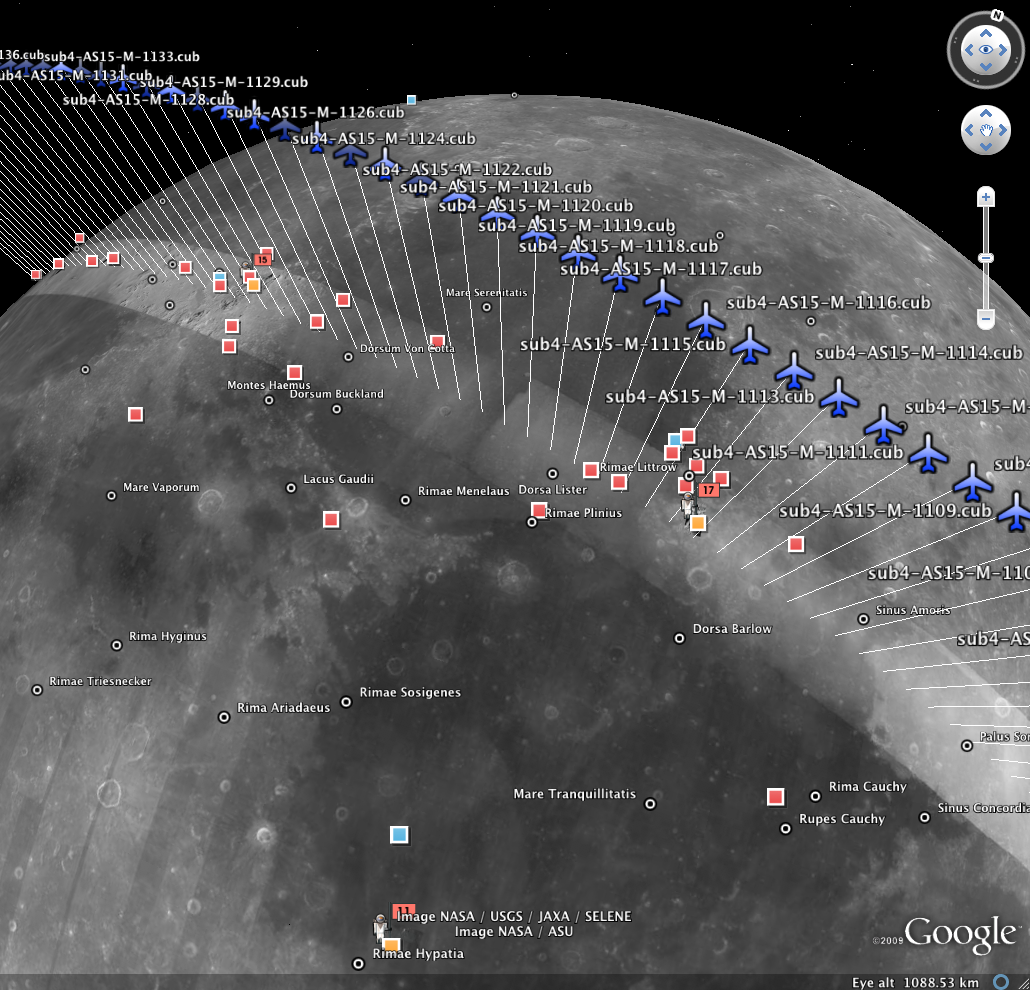
\includegraphics[width=6in]{images/orbitviz_ge_result.png}
  \end{center}
  \caption{ Example of a KML produced with orbitviz showing the location where cube files where taken. }
  \label{fig:orbitviz_example}
\end{figure}

\begin{longtable}{|l|p{10cm}|}
\caption{Command-line options for orbitviz}
\label{tbl:orbitviz}
\endfirsthead
\endhead
\endfoot
\endlastfoot
\hline
Options & Description \\ \hline \hline
\verb#--help# & Display this table \\ \hline
\verb#-o arg (=orbit.kml)# & Specifies the output file name \\ \hline
\verb#-s arg (=1)# & Scale the size of the coordinate axes by this amount. Ex: To scale alt. measures up to earth size, use 3.66 \\ \hline
\verb#-t# & Slect the stereo session type to use for processing. [default: pinhole] \\ \hline
\verb#--use-simple-placemarks# & Draw simple icons at camera locations, instead of a coordinate model \\ \hline
\end{longtable}

\section{orthoproject}
\label{orthoproject}

Map projects imagery on to point clouds.

Example:
\begin{verbatim}
orthoproject -t isis filename-DEM.tif filename.cub filename.isis_adjust \\
        filename-DRG.tif --nodata -10000 --ppd 256
\end{verbatim}

\begin{longtable}{|l|p{10cm}|}
\caption{Command-line options for orthoproject}
\label{tbl:orthoproject}
\endfirsthead
\endhead
\endfoot
\endlastfoot
\hline
Options & Description \\ \hline \hline
\verb#--help# & Display this table \\ \hline
\verb#--mpp arg# & Specify the output resolution of the orthoimage in meters per pixel \\ \hline
\verb#--ppd arg# & Specify the output resolution of the orthoimage in pixels per degree \\ \hline
\verb#--nodata-value arg# & Specify the pixel used in this DEM to denote missing data \\ \hline
\verb#-m# & Match the georeferencing parameters and dimensions of the input DEM \\ \hline
\verb#--min arg# & Explicitly specify the range of the normalization (for ISIS images only) \\ \hline
\verb#--max arg# & Explicitly specify the range of the normalization (for ISIS images only) \\ \hline
\verb#--cache arg# & Cache size, in megabytes \\ \hline
\verb#-t arg (=pinhole)# & Select the stereo session type to use for processing. [default: pinhole] \\ \hline
\verb#-d arg (=29)# & Set the debugging output level. (0-50+) \\ \hline
\end{longtable}

\section{point2dem}
\label{point2dem}

Produces a GeoTIFF terrain model or an orthographic image depending on the input flags.

This produces: 
	p19-DEM.tif - A DEM with floating point pixels. This is suitable for use in a GIS.
	p19-DEM-normalized.tif - A version of the DEM where the heights have been mapped onto the range 0-255 so that it can be viewed in a normal image viewer.

Example:
\begin{verbatim}
point2dem filename-PC.tif -o stereo/filename --xyz -r moon \\
        --default-value -10000
\end{verbatim}

\begin{longtable}{|l|p{10cm}|}
\caption{Command-line options for point2dem}
\label{tbl:point2dem}
\endfirsthead
\endhead
\endfoot
\endlastfoot
\hline
Options & Description \\ \hline \hline
\verb#--help# & Display this table \\ \hline
\verb#--default-value# & Explicitly set the default missing pixel value. By default, the min z value is used. \\ \hline
\verb#--use-alpha# & Create images that have an alpha channel \\ \hline
\verb#-s arg(=0)# & Set the DEM post size (if this value is 0, the post spacing size is computed for you) \\ \hline
\verb#-n# & Also write a normalized version of the DEM (for debugging) \\ \hline
\verb#--orthoimage arg# & Write an orthoimage based on the texture file given as an argument to this command line option \\ \hline
\verb#--grayscale# & Use grayscale image processing for creating the orthoimage \\ \hline
\verb#--offset-files# & Also write a pair of ascii offset files (for debugging) \\ \hline
\verb#--cache arg (=2048)# & Cache size, in megabytes \\ \hline
\verb#--input-file arg# & Explicitly specify the input file \\ \hline
\verb#--texture-file arg# & Explicitly specify the texture file \\ \hline
\verb#-o arg# & Specify the output prefix \\ \hline
\verb#-t arg (=tif)# & Specify the output file type \\ \hline
\verb#-d arg (=29)# & Set the debugging output level. (0-50+) \\ \hline
\verb#--xyz-to-lonlat# & Convert from XYZ coordinates to LLA coordinates \\ \hline
\verb#-r arg# & Set a reference surface to a hard coded value (one of [mmon, mars]). This will override manually set datum information. \\ \hline
\verb#--semi-major-axis arg (=0)# & Set the dimensions of the datum \\ \hline
\verb#--semi-minor-axis arg (=0)# & Set the dimensions of the datum \\ \hline
\verb#--x-offset arg (=0)# & Add a horizontal offset to the DEM \\ \hline
\verb#--y-offset arg (=0)# & Add a horizontal offset to the DEM \\ \hline
\verb#--z-offset arg (=0)# & Add a vertical offset to the DEM \\ \hline
\verb#--sinusoidal# & Save using a sinusoidal projection \\ \hline
\verb#--mercator# & Save using a Mercator projection \\ \hline
\verb#--transverse-mercator# & Save using transverse Mercator projection \\ \hline
\verb#--orthographic# & Save using an orthographic projection \\ \hline
\verb#--stereographic# & Save using a stereographic projection \\ \hline
\verb#--lambert-azimuthal# & Save using a Lambert azimuthal projection \\ \hline
\verb#--utm arg# & Save using a UTM projection with the given zone \\ \hline
\verb#--proj-lat arg# & The center of projection latitude (if applicable) \\ \hline
\verb#--proj-lon arg# & The center of projection longitude (if applicable) \\ \hline
\verb#--proj-scale arg# & The projection scale (if applicable) \\ \hline
\verb#--rotation-order arg (=xyz)# & Set the order of an euler angle rotation applied to the 3D points prior to DEM rasterization \\ \hline
\verb#--phi-rotation arg (=0)# & Set a rotation angle phi \\ \hline
\verb#--omega-rotation arg (=0)# & Set a rotation angle omega \\ \hline
\verb#--kappa-rotation arg (=0)# & Set a rotation angle kappa \\ \hline
\end{longtable}

\section{point2mesh}
\label{point2mesh}

Produces a mesh surface which can be visualized in
OpenSceneGraph. This is not meant to produce a finished scientific
product, this is only for fast visualization and to create a cool 3D
view of the data generated. \verb#point2mesh# requires a point cloud
file and optionally a left texture file \emph{(as the left texture is
  from the same perspective as the point cloud)}. When a texture is
not provided, a 1D texture is applied in the local Z direction. That
produces a rough rendition of a contour map.

This will produce two files, a \verb#*.ive# which is the 3D model and
an additional \verb#*.tif# that is the reduced texture used on the
model. This texture file is not need after it's creation and is only a
device for interfacing with OpenSceneGraph.

Two other important options to know about are the flags \verb#-l# and
\verb#-s arg#. The first provides light to be calculated on the model,
thus when in \verb#osgviewer# it is easier to see the texture of the
model. The last flag mention is the sampling rate. The default value
is 10, meaning every 10th point is used in the X and Y directions. In
other words that mean only $1/10^2$ of the points are being used to
create the model. Adjust this sampling rate accordingly to see the
amount of the detail wanted, but high enough so as not to hurt
framerate.

Example:
\begin{verbatim}
      point2mesh -l -s 2 output-PC.tif output-L.tif
\end{verbatim}

To view the resulting \verb#*.ive#, use \verb#osgviewer#

\begin{verbatim}
      # Fullscreen
      osgviewer output.ive
      # or Windowed
      osgviewer output.ive --window 50 50 1000 1000
\end{verbatim}

Inside \verb#osgviewer#, the keys L, T, and W can be used to toggle on
and off lighting, texture, and wireframe.

\begin{longtable}{|l|p{10cm}|}
\caption{Command-line options for point2mesh}
\label{tbl:point2mesh}
\endfirsthead
\endhead
\endfoot
\endlastfoot
\hline
Options & Description \\ \hline \hline
\verb#--help# & Display this table \\ \hline
\verb#--simplify-mesh arg# & Run OSG Simplifier on mesh, 1.0 = 100\% \\ \hline
\verb#--smooth-mesh# & Run OSG Smoother on mesh \\ \hline
\verb#--use-delaunay# & Uses the delaunay triangulator to create a surface from the point cloud. This is not recommended for point clouds with noise issues. \\ \hline
\verb#-s arg (=10)# & Sampling step size for mesher. \\ \hline
\verb#--input-file arg# & Explicitly specify the input file \\ \hline
\verb#--texture-file arg# & Explicitly specify the texture file \\ \hline
\verb#-o arg# & Specify the output prefix \\ \hline
\verb#-t arg (=ive)# & Specify the output file type \\ \hline
\verb#-l# & Enables shades and light on the mesh \\ \hline
\verb#--center# & Center the model around the origin. Use this option if you are experiencing numerical precision issues. \\ \hline
\verb#--rotation-order arg (=xyz)# & Set the order of an euler angle rotation applied to the 3D points prior to DEM rasterization \\ \hline
\verb#--phi-rotation arg (=0)# & Set a rotation angle phi \\ \hline
\verb#--omega-rotation arg (=0)# & Set a rotation angle omega \\ \hline
\verb#--kappa-rotation arg (=0)# & Set a rotation angle kappa \\ \hline
\end{longtable}

\section{reconstruct}
\label{reconstruct}

Tool under development

\section{results}
\label{results}

Tool under development

\section{rmax\_adjust}
\label{ramx_adjust}

Bundle Adjustment tool specifically for the Yamaha RMAX unmanned
aerial vehicle.

\section{stereo}
\label{stereo}

The \texttt{stereo} program is the primary workhorse of the Ames
Stereo Pipeline.  It is the program that takes a pair of images which
overlap and creates an output point cloud which can then be fed to the
\texttt{point2mesh} or \texttt{point2dem} programs.

\medskip

Usage:
\begin{verbatim}
    stereo [options] <Left_input_image> <Right_input_image> \\
           [Left_camera_file] [Right_camera_file] <output_file_prefix>
\end{verbatim}

\medskip

In principal, the stereo program is very simple, it takes two input
images (and their optional camera files) and creates a bevy of
output files.

The \verb=<Left_input_image>= and \verb=<Right_input_image>= files can be a wide variety of image formats.  If your input image files contain camera information (e.g. ISIS \verb=.cub= files), then the \verb=Left_camera_file= and \verb=Right_camera_file= are optional.

When working with data that doesn't have camera information embedded
in the file, camera information must be supplied in a format
understood by Vision Workbench's Camera Module. The formats accepted
there are pinhole models via the \verb#.tsai# and \verb#.pinhole#
extension, and CAHV/CHAVOR. Again this only important when working sessions
other than ISIS.

The \verb=<output_file_prefix>= is what \verb=stereo= uses as the
beginning part of most of the files that it writes out.  If you set
\verb=<output_file_prefix>= to be `\verb=out=' then files will be
named \verb=out-L.tif= and  \verb=out-PC.tif=.  If you use something
like `\verb=out/out=' for \verb=<output_file_prefix>= then the
\verb=stereo= program will create a directory called \verb=out/= and
place files named \verb=out-L.tif=, \verb=out-PC.tif=, etc. into
that directory, which can sometimes be handy.

\begin{longtable}{|l|p{10cm}|}
\caption{Command-line options for stereo}
\label{tbl:stereo}
\endfirsthead
\endhead
\endfoot
\endlastfoot
\hline
Option & Description \\ \hline \hline
\verb#--help# & Display this table\\ \hline
\verb#--cache arg (=1800)# & Set the maximium cache available in megabytes\\ \hline
\verb#--threads arg (=0)# & Set the number threads to use. 0 means use default defined .vwrc\\ \hline
\verb#--session-type arg# & Select the stereo session type to use for processing. Usually the program can select this automatically for file extension. [options pinhole isis]\\ \hline
\verb#--stereo-file arg (=./stereo.default)# & Define the stereo.default file to use\\ \hline
\verb#--entry-point# & Pipeline entry point [options 1-4]\\ \hline
\verb#--debug-level# & Sets the output debugging level\\ \hline
\verb#--draft-mode arg# & Cause the pyramid correlator to save out debug imagery named with this prefix\\ \hline
\verb#--optimized-correlator# & Cause scale space search to not be performed\\ \hline
\end{longtable}

\subsection{Entry Points}
\label{entrypoints}

Stage 0 (Preprocessing) normalizes the two images and aligns them
(thus non-projected images are easier to work with) by locating
interest points and matching them in both images. The program is
designed to reject outlying interest points.  This stage writes out
the pre-aligned images and the image masks.

Stage 1 (Correlation) performs the image correlation and the building
of a disparity map.

Stage 2 (Refinement) performs sub-pixel correlation which further
refines the solution.

Stage 3 (Filtering) performs filtering of the disparity map and
creates a ``good pixel'' map.  If enabled, this is also the step
where holes are filled in.

Stage 4 (Triangulation). The disparity map is processed to remove
the effects of interest point alignment and a 3D point cloud is
created.

